

\begin{frame}{Benefits of Linear RNNs}
    \begin{itemize}
        \item Methods for training (CNN) and generation (RNN)
        \item Potentially more FLOP efficient. 
        \item However not yet used in practice 
    \end{itemize}    
\end{frame}

\begin{frame}[c]{Current Efficiency with Scale \cite{Poli2023-ag}}
\begin{figure}
    \centering
    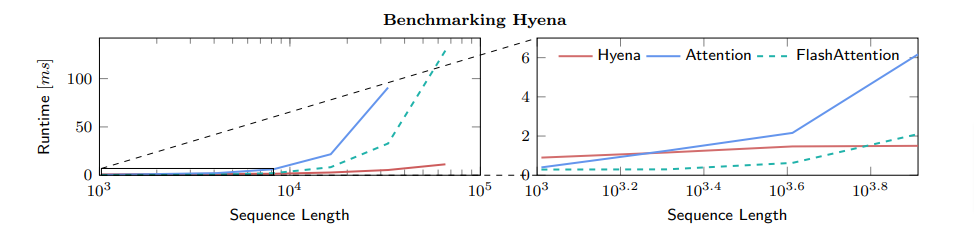
\includegraphics[width=\textwidth]{Figs/hyena.png}
    \caption{}
\end{figure}
 Models become more efficient at long time-scales.
\end{frame}

\begin{frame}{Issues on Accelerators}
    Approaches require:
    \vspace{0.5cm}

    \begin{itemize}
        \item Support for complex numbers
        \item Support for FFT (lower precision, TPU)
        \item Numerical Stability
        \item Fast Associative Scans 
    \end{itemize}
    \vspace{0.5cm}
    
    Hard to compete with pure MatMul in Attention.
\end{frame}

\begin{frame}{}
    \begin{figure}
        \centering
        
\includegraphics[width=0.7\linewidth,clip,  trim={0.1cm 0.1cm 0.1cm 0.1cm}]{Figs/Is-Attention-All-You-Need-.png}
        \label{fig:my_label}
    \end{figure}
\end{frame}


% \begin{frame}{Frame Title}
%     Call to action. 

%     * Modeling benefits
%     * Theoretical approaches
%     * interplay with hardware efficiency. 
%     * Matching transformers 
%     * FFT / Complex 
%     * Associative scans
%     * GPU / TPUs 
%     * Models are more flop efficient, FLOPs are not equal. 
%     * Matmuls are more efficienct. 
%     * Numerical stability / complex numbers 
%     * 
% \end{frame}




% \begin{frame}{State Retrieval}
%     \begin{itemize}
%         \item Benchmarks compare perplexity of models
%         \item Significant interest is in abilities such as in-context learning
%         \item Current understanding relies of set-based Transformer mechanisms.
%     \end{itemize}
% \end{frame}




% \begin{frame}{In-Context Learning}
%     \begin{itemize}
%         \item Benchmarks compare perplexity of models
%         \item Significant interest is in abilities such as in-context learning
%         \item Current understanding relies of set-based Transformer mechanisms.
%     \end{itemize}
% \end{frame}

% \begin{frame}{Better Transformers}
%     \begin{itemize}
%         \item Models are being scaled to longer ranges (>100k)
%         \item For language, approximations of attention may be fine.
%         \item 
%     \end{itemize}
% \end{frame}


% \begin{frame}{Inductive Bias}
%     \begin{itemize}
%         \item Transformers are set-based models 
%         \item Linear RNNs encoder sequential bias
%         \item For language, unclear whether this is beneficial or not.
%     \end{itemize}
% \end{frame}